\label{sec:method}

We target \emph{posture-requested} one-shot personalization: from a single reference image $I_{\mathrm{id}}$ of an identity and a posture request $p$, generate an image of \emph{that} identity at posture $p$. The text prompt is not a bare pose command: it carries the same scene, attire, and style detail an ordinary T2I prompt would, since posture control has to hold up embedded in a full generation, not only in isolation. These two items---$I_{\mathrm{id}}$ and $p$---are the \emph{only} inputs the user provides; every other signal the pipeline uses internally, including the structural pose control introduced in Sec.~\ref{sec:pose}, is constructed by the system itself from $p$, never supplied externally.

\paragraph{One generation, end to end.} Before any detail, here is the whole pipeline in four sentences (follow Fig.~\ref{fig:backbone_arch}). The posture prompt, the noise canvas, three copies of the \emph{single} reference face, and a pose skeleton---\emph{built by the system from that same prompt, Sec.~\ref{sec:pose}, never supplied by the user}---are each encoded into tokens and concatenated into \emph{one} sequence. A frozen transformer runs joint attention over that sequence for four denoising steps; whatever share of attention the face tokens win is how much identity survives. Our method is, at heart, the management of that share: a skeleton makes the head turn, duplication wins identity back, and a $\sim$200-parameter learned gate ($\gamma$-gate) tunes the share precisely---the backbone itself is never trained. The chapter unfolds in that order: the shared substrate (Sec.~\ref{sec:backbone}), \emph{making the head turn} (Sec.~\ref{sec:pose}), \emph{keeping the face} (Sec.~\ref{sec:identity}), and \emph{learning the budget} (Sec.~\ref{sec:learned}); Sec.~\ref{sec:whyworks} then verifies causally \emph{why} these levers work. This walkthrough already
leaned on shorthand---duplication, the gate, the attention budget---that
recurs for the rest of the chapter and into the experiments; Table~\ref{tab:terms}
fixes each term precisely, for reference as they reappear.

\begin{table}[t]\centering\small
\setlength{\tabcolsep}{5pt}
\adjustbox{max width=\linewidth}{%
\begin{tabular}{@{}ll@{}}
\toprule
term & meaning \\
\midrule
\dupid & repeat the identity token block $N$ times ($N{=}3$), placed first \\
\emph{id-first} & reference order $[C_{\mathrm{id}}{\times}N,\,C_S]$ (identity before skeleton) \\
\gate & learned per-(step, layer) gain on a block's attention ($\sim$200 params) \\
PAEs & pose-\emph{adapted} face encoders: identity read by yaw-matched experts \\
$\widetilde{\mathrm{CSIM}}(k)$ & pose-\emph{aware} identity: $\mathrm{CSIM}\cdot e^{-k(1-\mathrm{Acc_{yaw}})}$ (Eq.~\ref{eq:posepenalty}) \\
OTS & over-the-shoulder: head turned far relative to the torso ($|\Delta\theta_y|{>}25^\circ$) \\
\bottomrule
\end{tabular}}
\caption[Terminology]{\textbf{Terminology} used throughout this chapter and the experiments.}
\label{tab:terms}
\end{table}

\section{The backbone and its in-context conditioning}
\label{sec:backbone}
FLUX.2-klein~\cite{flux2} is a guidance-distilled, few-step (4-step)
rectified-flow~\cite{rectifiedflow,flowmatching} multimodal DiT (MM-DiT~\cite{sd3}):
training regresses the flow-matching target
$\mathcal{L}_{\mathrm{fm}}=\mathbb{E}\,\lVert v_\theta(x_\sigma,\sigma,c)-(\epsilon-x_0)\rVert_2^2$
with $x_\sigma=(1-\sigma)x_0+\sigma\epsilon$, and sampling is four Euler steps
with no classifier-free guidance. Three components fix every dimension we use
later (all details in Fig.~\ref{fig:backbone_arch}): \textbf{(a)}~a 32-channel
VAE ($8\times$ down) followed by a $2{\times}2$ patchify turns any image into
$N{=}(H/16)(W/16)$ tokens of $128$ channels ($512^2\!\rightarrow\!1{,}024$
tokens; $1024^2\!\rightarrow\!4{,}096$), lifted linearly to the model width;
\textbf{(b)}~the prompt passes a frozen Qwen3-4B whose stacked hidden layers
$(9,18,27)$ give $7{,}680$-dim features, projected to the same width---so
\emph{text tokens live in the same sequence as image tokens and compete for the
same attention}; \textbf{(c)}~the trunk stacks $5$ double-stream and $20$
single-stream blocks---$L{=}25$ attention layers, $24$ heads $\times\,128$ dims
($d{=}3072$)---each computing one \emph{joint} self-attention
$\mathrm{softmax}(QK^{\!\top}/\sqrt{d_h})V$ over the full sequence, with no
cross-attention branch. These $4\times25=100$ (step,\,layer) attention sites are
exactly where the allocator of Sec.~\ref{sec:learned} attaches.

\begin{figure}[t]\centering
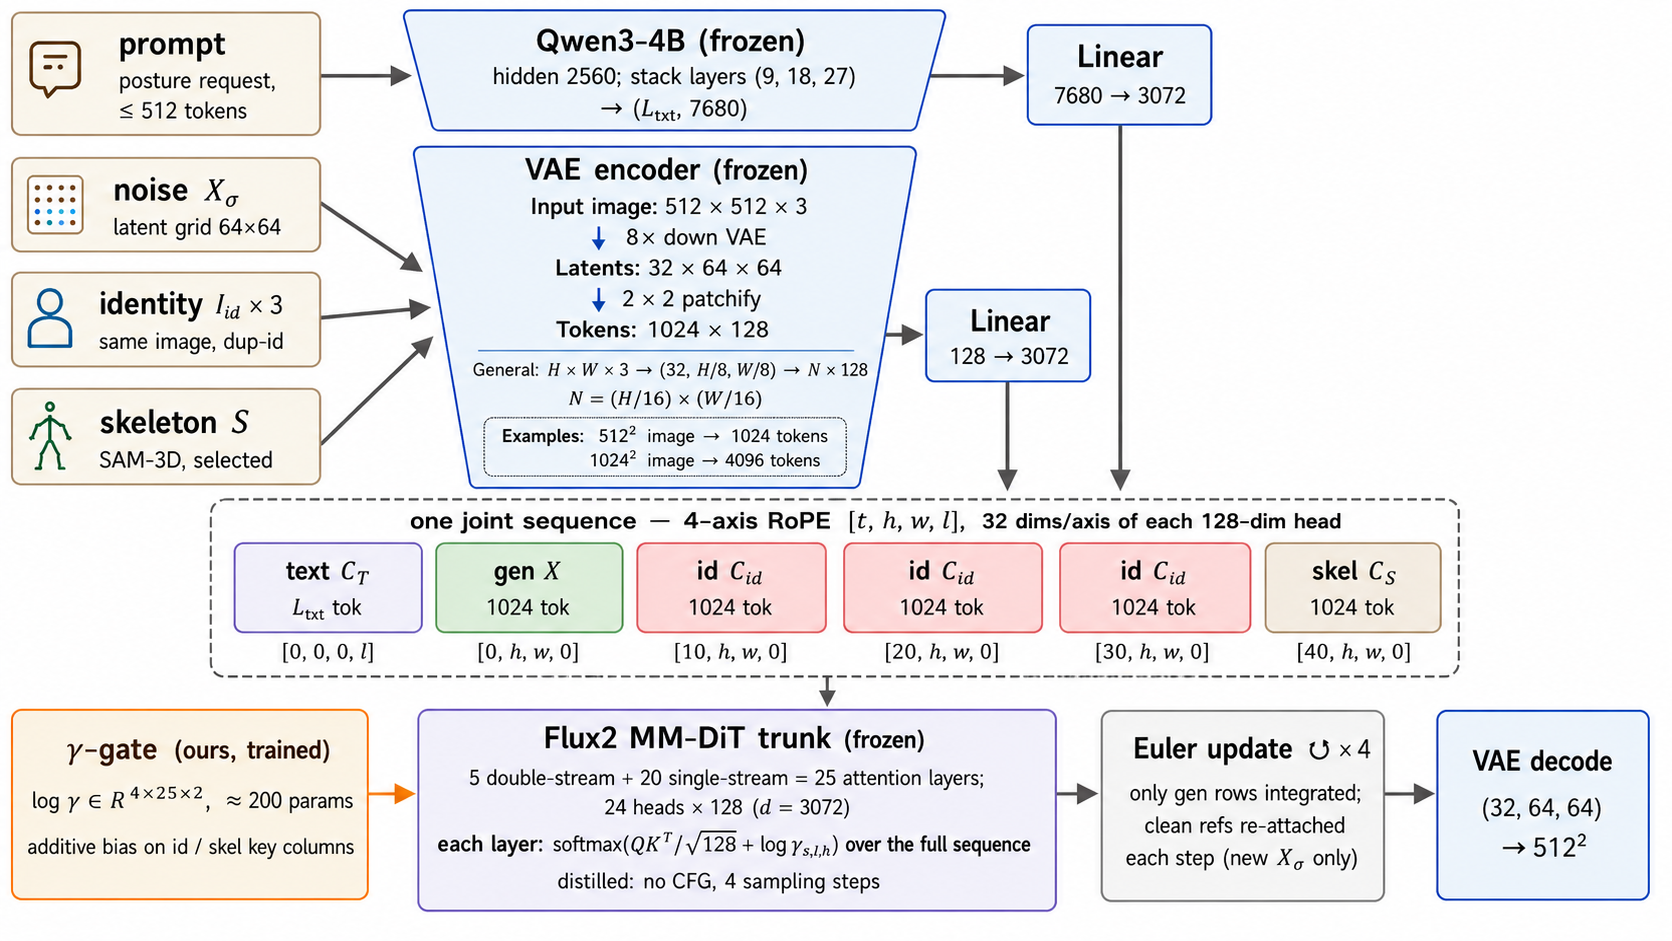
\includegraphics[width=\textwidth]{figures/pipeline_wRoPE.png}
\caption[The FLUX.2-klein-4B backbone with full dimensions]{\textbf{The FLUX.2-klein-4B backbone with full dimensions}
(Sec.~\ref{sec:backbone}; $512^2$ example). All image inputs share one frozen
VAE$+$patchify path; all segments meet in one joint sequence whose RoPE
coordinates $[t,h,w,l]$ (below each block) separate the reference copies on the
$t$-axis and make list order positional. The \gate{} (gold) adds
$\log\gamma_{s,\ell,k}$ to the identity/skeleton key columns of every joint
attention; four Euler steps integrate only the generation rows.}
\label{fig:backbone_arch}
\end{figure}

\paragraph{Reference tokens: one sequence.}
\label{sec:refgeometry}
Conditioning is \emph{in context}: each reference or control image is VAE-encoded
and patchified by the \emph{same} path as the generation target and concatenated
as a block of latent tokens into one sequence with the noisy generation, so a
single joint self-attention mixes text, generated, and reference tokens:
\begin{equation}
\big[\,\underbrace{X}_{\text{gen}}\,\;\underbrace{C_T}_{\text{text}}\,\;\underbrace{C_{\mathrm{id}}\;C_S}_{\text{reference blocks}}\big],
\end{equation}
where $X$ are the \emph{noisy generation tokens} $x_\sigma$ being denoised---the
in-progress canvas the network predicts, \emph{not} a previously generated image
fed back in---and the conditioning $c$ in $\mathcal{L}_{\mathrm{fm}}$ is the text
$C_T$ together with the reference blocks $\{C_{\mathrm{id}},C_S\}$, the token
embeddings of the identity image $I_{\mathrm{id}}$ and the structural control
$S$. The generator is given \emph{two} kinds of reference block, of different
provenance: the \emph{identity} image $I_{\mathrm{id}}$ (tokens
$C_{\mathrm{id}}$, for appearance)---the user's one input---and a
\emph{structural} control $S$ (tokens $C_S$, for pose), which the system
\emph{constructs} from the posture request $p$ (Sec.~\ref{sec:pose}) rather
than receiving from the user. In-context conditioning reuses the backbone's
own weights on the concatenated tokens---unlike a ControlNet or adapter branch it
adds essentially no parameters~\cite{ominicontrol}---so personalization stays
efficient under the 4-step sampler.

\paragraph{Where each token \emph{sits}: 4-axis RoPE.} FLUX.2 distinguishes the
segments not by learned embeddings but by \emph{rotary position coordinates} on
four axes $(t,h,w,l)$, each allotted $32$ of the $128$ head dimensions. Text
tokens occupy $[0,0,0,l]$ (only the sequence axis $l$ advances); generation
tokens occupy $[0,h,w,0]$ on their latent grid; and the $i$-th reference block is
placed at
\begin{equation}
[\,t,h,w,l\,]=[\,s\,(1+i),\,h,\,w,\,0\,],\qquad s{=}10 ,
\label{eq:ropeids}
\end{equation}
i.e.\ references share the generation's spatial grid but are pushed down a
virtual \emph{time} axis at $t=10,20,30,\dots$ in list order. Two consequences
drive this paper. \emph{First}, all conditioning---text, identity,
structure---meets the generation in the \emph{same} softmax, so conditioning
strength is a zero-sum share of one attention budget (Sec.~\ref{sec:mechanism}).
\emph{Second}, the $t$-axis makes reference \emph{order} a real variable under
RoPE's relative-distance decay---a geometric fact Sec.~\ref{sec:identity} puts
to direct use.

\paragraph{How references persist across steps.} At every denoise step the
\emph{clean} reference latents are re-concatenated unchanged behind the current
noisy state ($\mathrm{cat}[x_\sigma;\,C_{\mathrm{id}};C_S]$); only the generation
rows are integrated by the sampler, the velocity prediction being sliced back to
the first $|X|$ tokens. References are never noised and never denoised---they are
pure context, read afresh at each of the four steps. (Because their keys/values
are constant across steps, implementations may cache reference K/V once and reuse
it; we keep them in-sequence, which is what makes the per-step, per-layer
budget analysis and the allocator of Sec.~\ref{sec:learned} possible.) The
backbone is \textbf{frozen throughout}; our only trainable component is the
small allocator of Sec.~\ref{sec:learned}. Because references are just
key/value blocks in this one softmax, everything that can strengthen identity
without touching a weight is a re-weighting of that shared budget---which is
the thread the rest of this chapter pulls on, and which Sec.~\ref{sec:whyworks}
verifies causally.

\section{Making the head turn: selecting the structural pose control}
\label{sec:pose}

\paragraph{Constructing the pose control.} The structural control $S$ that drives
rotation is never supplied by the user---the pipeline builds it automatically
from the posture request $p$, in four stages; the last feeds the generator of
Fig.~\ref{fig:backbone_arch}. \textbf{(a)~Synthesize.} We generate a pool of candidate
person images with the FLUX.2-klein backbone prompted for the target head pose.
\textbf{(b)~Measure and filter.} Because a T2I model does \emph{not} reliably
realize a requested out-of-plane pose, we do not trust the prompt: we estimate
the actual pose of every candidate with SMPLest-X~\cite{smplestx}---reading head
yaw $\theta_y$, head pitch $\theta_p$, and the head-to-torso yaw
$\Delta\theta_y$---and classify it by the same pose categories and thresholds we
use for evaluation (defined in Sec.~\ref{sec:metrics}), discarding candidates whose
\emph{measured} pose does not match the intended category. \textbf{(c)~Extract control.} From each retained image we
predict a body and render a control map---our choice is a projected
SAM-3D-Body~\cite{sam} keypoint skeleton (justified in
Table~\ref{tab:featuremap}); mesh-depth, surface-normal, and SMPL-X-skeleton
alternatives are rendered the same way for comparison. \textbf{(d)~Guide.} The
selected control $S$ is concatenated \emph{in context} with the single identity
image and drives the generator (Sec.~\ref{sec:identity}). The rest of this
subsection establishes the backbone, justifies the control choice in~(c), and
gives the per-category selection rule used in~(b).

\paragraph{Backbone.} We build on FLUX.2-klein, which attains the best
text-driven head rotation among six T2I backbones we benchmark
(App.~\ref{sec:appendix_backbone}, Table~\ref{tab:backbone}). Even this strongest
backbone tops out at $67.5\%$ yaw and rarely reaches profile from text alone,
establishing that prompting cannot reliably realize out-of-plane rotation---the
motivation for the explicit structural control we develop next.

\paragraph{Which structural control?} We render four in-context controls from a
fitted body model and compare how faithfully each \emph{transfers} a target head
orientation: a dense surface-\emph{normal} map, a mesh-\emph{depth} map, a 2D
projected SMPL-X~\cite{smplestx} \emph{skeleton}, and a SAM-3D-Body~\cite{sam}
70-keypoint skeleton (``sam3d''). Table~\ref{tab:featuremap} reports yaw mean
absolute error and yaw/pitch direction accuracy. The sparse \textbf{sam3d
skeleton} transfers orientation best (lowest yaw error, highest pitch
direction accuracy): dense maps over-constrain appearance and blur the head
axis, whereas an explicit keypoint skeleton carries head orientation cleanly.

\begin{table}[t]\centering\small
\setlength{\tabcolsep}{5pt}
\adjustbox{max width=\linewidth}{%
\begin{tabular}{lccc}
\toprule
Structural control & Yaw MAE\,$\downarrow$ & Yaw dir.\,$\uparrow$ & Pitch dir.\,$\uparrow$ \\
\midrule
\textbf{sam3d skeleton}~\cite{sam} & \textbf{28.2} & \textbf{80.3} & \textbf{75.6} \\
% skeleton (SMPL-X)~\cite{smplestx} & 34.9 & 72.1 & 72.6 \\
surface-normal & 39.3 & 68.7 & 72.4 \\
mesh-depth & 39.4 & 68.6 & 72.4 \\
\bottomrule
\end{tabular}}
\caption[Which in-context structural control transfers head orientation best]{\textbf{Which in-context structural control transfers head orientation
best} (cross-pose transfer, $n{=}1560$ pairs/control; yaw MAE in degrees,
direction accuracy in \%). The sparse SAM-3D keypoint skeleton gives the lowest
yaw error and highest direction accuracy; dense surface maps over-constrain
appearance and blur the head axis. The \emph{do-nothing} yaw MAE is $52.5^\circ$.}
\label{tab:featuremap}
\end{table}

\paragraph{Verified skeleton selection.} The hardest sub-case is the
\emph{over-the-shoulder} (OTS) view, which the backbone resists. We observe that
FLUX renders OTS only for skeletons whose \emph{measured} head-to-torso yaw is
large, regardless of the skeleton's nominal caption. We therefore \emph{select},
per target category, the skeleton with the strongest measured head-to-torso yaw
in the matching turn direction (Fig.~\ref{fig:skeleton}); this purely
measurement-driven rule lifts full-benchmark yaw accuracy substantially over
using each prompt's own (often mis-posed) skeleton. The selected control is the
$S$ used below.

\begin{figure}[t]\centering
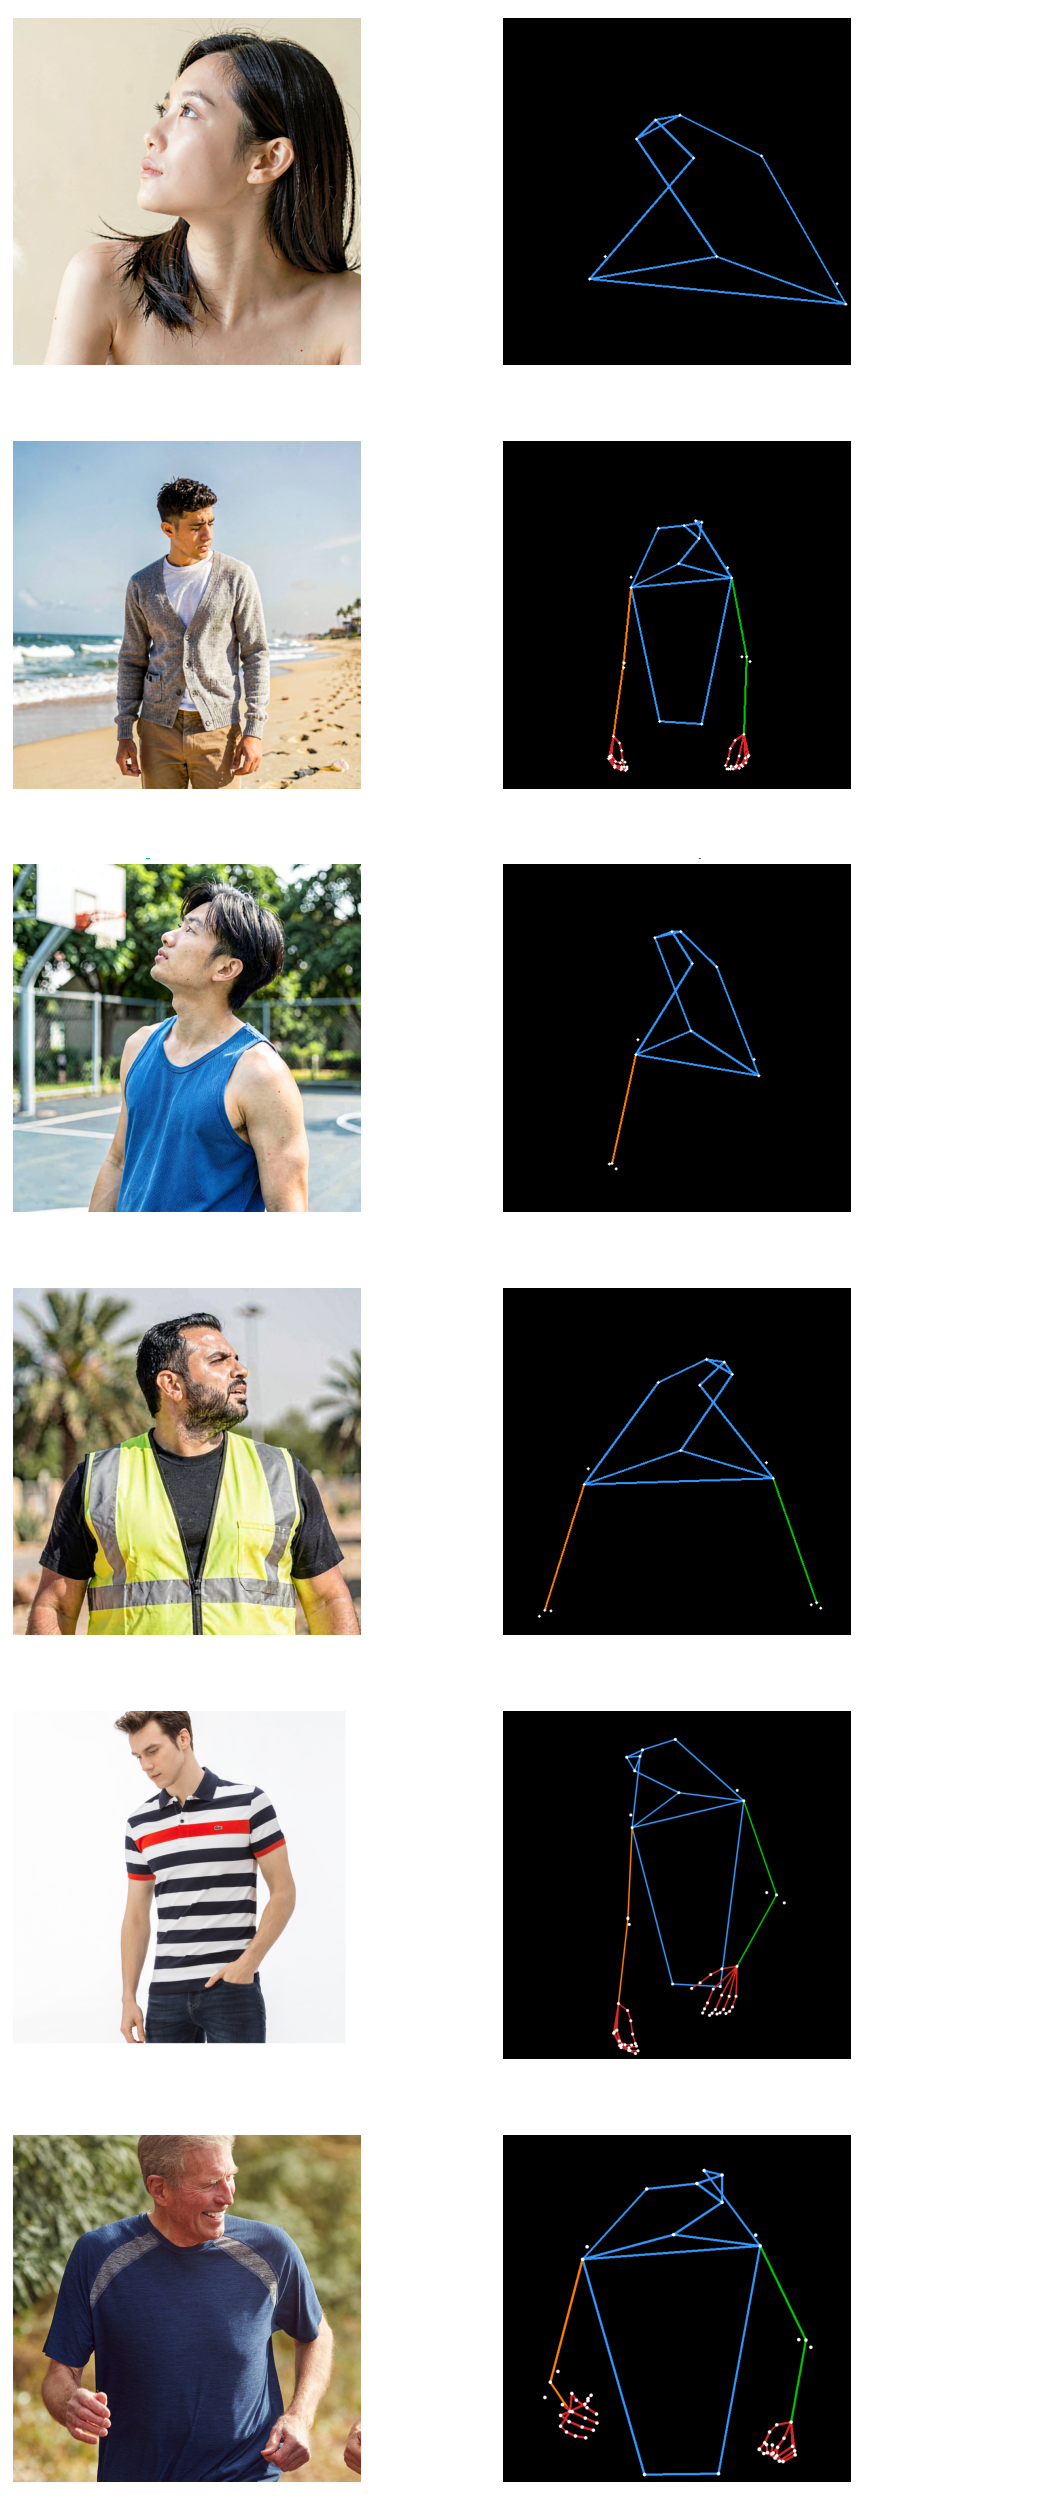
\includegraphics[width=0.8\linewidth]{figures/skeleton_templates.png}
\caption[Verified skeleton selection]{\textbf{Verified skeleton selection.} Per target pose category we select
the candidate skeleton whose \emph{measured} head-to-torso yaw is largest in the
matching turn direction, rather than the prompt's own (often mis-posed) skeleton.
This measurement-driven rule reliably triggers over-the-shoulder rendering, which
the backbone otherwise resists. Each row shows the source pose image (left) and the
selected SAM-3D skeleton fed to the generator (right); the six rows span left/right
over-the-shoulder and chin-up/chin-down.}
\label{fig:skeleton}
\end{figure}

\section{Keeping the face: reference duplication (\dupid)}
\label{sec:identity}
\paragraph{The pose--identity trade-off.} Adding the structural control sharpens
pose but \emph{lowers} identity similarity (\csim, AdaFace~\cite{adaface} cosine
to $I_{\mathrm{id}}$): the extra reference competes with the identity reference
for the generated tokens' attention. Recovering identity \emph{without} giving
back the pose gain is the problem we now solve.

\paragraph{Reference duplication and ordering (\dupid).} Since each reference is
a contiguous token block, we increase the identity block's influence simply by
\emph{repeating} its tokens $C_{\mathrm{id}}$ $N$ times and placing them \emph{first}:
\begin{equation}
\big[\,\underbrace{C_{\mathrm{id}},\dots,C_{\mathrm{id}}}_{N},\,C_S\,\big].
\label{eq:dupid}
\end{equation}
Duplication raises \csim{} sharply up to $N{=}3$; the \emph{id-first} ordering
is the key lever that retains pose while doing so. We keep the identity word in
the prompt (duplication overrides it), avoiding the brittle ``strip-identity''
alternative. Figure~\ref{fig:idemergence} shows the identity \emph{emerging}
as $N$ grows across three identities: without duplication the model often
renders the \emph{prompt's} nominal identity rather than the reference, and
pushing $N$ \emph{past} $3$ pays off unevenly---sometimes helping, sometimes
costing identity or pose---exactly why we refine $N{=}3$ with a learned gate
rather than simply increasing it further.

\begin{figure}[t]\centering
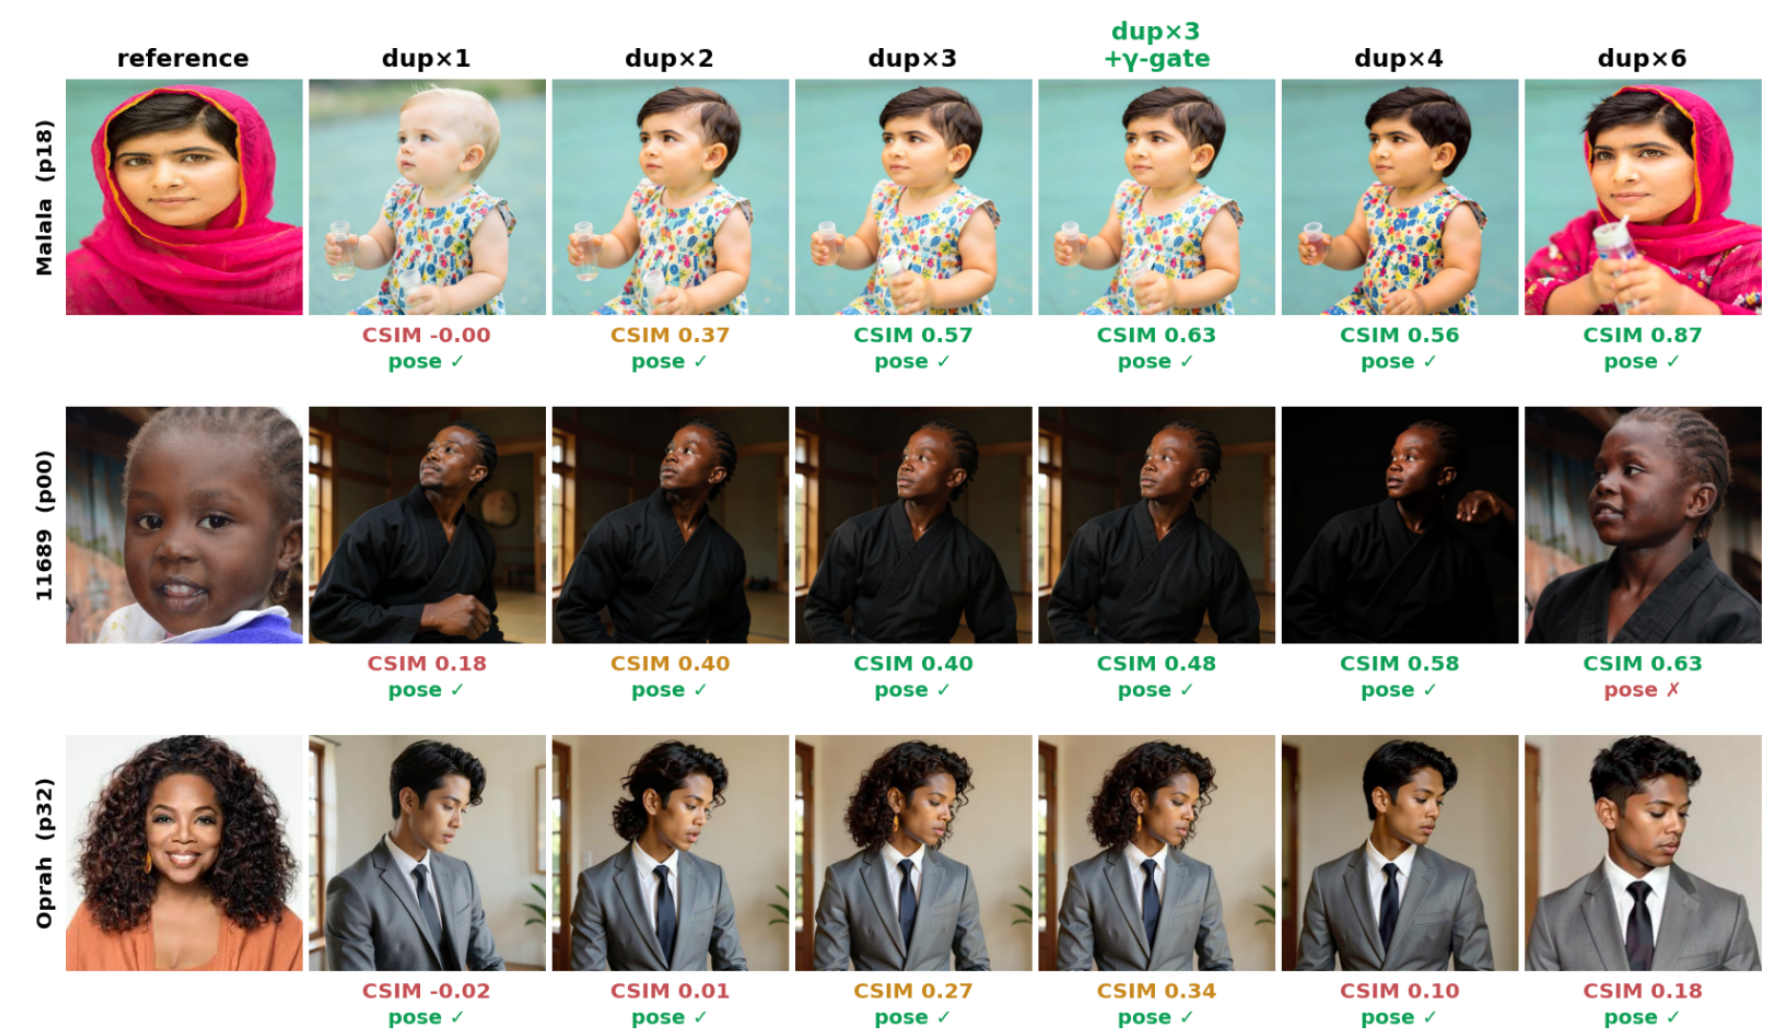
\includegraphics[width=\linewidth]{figures/id_emergence.png}
\caption[Identity emerges with duplication, and plateaus unevenly beyond $N{=}3$]{\textbf{Identity emerges with duplication, and plateaus unevenly
beyond $N{=}3$.} Three identities (rows), reference at left; each cell reports
\csim{} to the reference and whether the requested pose was met. At $N{=}1$
identity is weak or entirely wrong (row~1's generation is a different person);
duplication recovers it by $N{=}3$. Adding the \gate{} on top of $N{=}3$
(green) then gives a further, \emph{consistent} \csim{} gain in every row
($+0.06$ to $+0.08$) without ever losing pose. Pushing $N$ past $3$ instead is
unreliable: $N{=}4$ helps row~2 but collapses row~3's identity
($0.27\!\rightarrow\!0.10$), and $N{=}6$ gives row~1 its best \csim{} yet
breaks pose in row~2---the inconsistency that motivates \emph{learning} the
budget precisely (Sec.~\ref{sec:learned}) rather than hand-tuning $N$. Pushed
further still on a single case, $N$ eventually collapses into outright
copy-paste (Fig.~\ref{fig:visualprogress}).}
\label{fig:idemergence}
\end{figure}

\paragraph{From discrete levers to one learnable knob.} Duplication and ordering
raise identity but are coarse, discrete controls; Sec.~\ref{sec:learned}
replaces them with a learned, prompt-faithful gate that \emph{refines}
duplication. Sec.~\ref{sec:mechanism} then shows both---duplication and the
gate---are one and the same operation on the joint-attention budget; this
duplication-plus-gate is the Rotate-ID configuration reported throughout.

\paragraph{Reading identity at profile.} AdaFace \csim{} falls from frontal to
profile for \emph{every} configuration (Sec.~\ref{sec:exp_id}); we argue this
drop is largely a property of the \emph{recognizer}, not of the generations.
AdaFace is trained on near-frontal data, so a frontal-referenced cosine
\emph{under}-reads identity exactly where we operate~\cite{pasl}. Three
independent checks---the pose-adapted metrics read-out, cross-encoder agreement,
and the frontal-to-profile drop measured between \emph{real} photographs of the
same person (the CFP gap~\cite{cfp})---separate the metric artifact from real
loss; the full argument is in App.~\ref{sec:appendix_profile}. Under the
pose-adapted read-out, Rotate-ID holds identity as the head turns, whereas the
baselines do not reach the profile regime at all.

\section{Learning the budget: the \gate{} allocator}
\label{sec:learned}
Duplication and ordering are coarse, discrete controls on the same identity
attention share---so we make the control \emph{learnable} instead. We attach a
tensor of log-gains
$\log\gamma\in\mathbb{R}^{S\times L\times K}$ indexed by denoise step $S{=}4$,
attention layer $L{=}25$, and block kind $K{\in}\{\mathrm{id},\mathrm{skel}\}$
($\sim$200 parameters), and add $\log\gamma_{s,\ell,k}$ to the corresponding
block's columns at step $s$, layer $\ell$. Initialized at $\log\gamma{=}0$
($\gamma{=}1$), the model \emph{starts exactly at the \dupid{} configuration}, so
training can only depart from a strong baseline. The backbone is frozen; the
allocator is the only trainable object. (Sec.~\ref{sec:whyworks} verifies
causally that this log-gain intervention reproduces duplication's effect via
the identical mechanism---attention re-allocation, not added token capacity.)

\paragraph{Leakage-free objective.} A one-step identity loss is gameable---the
target leaks through the low-noise latent, so the gates can lower it without
learning to \emph{use} the identity. We instead generate from pure noise through
the differentiable 4-step sampler with the gates active, decode, detect and align
the face, run frozen AdaFace, and penalize
\begin{equation}
\mathcal{L}=\underbrace{\big(m-\cos(f_{\mathrm{gen}},f_{\mathrm{id}})\big)_{+}}_{\text{margin-clamped identity}}+\;\lambda\,\overline{(\log\gamma)^2},
\label{eq:gateloss}
\end{equation}
with a small regularizer pulling the gates toward the winner (protecting pose and
quality). From noise there is no leakage, so the only way to raise the cosine is
to actually route attention to the identity. We \emph{freeze the skeleton gain}
($\gamma_{\mathrm{skel}}{=}1$) so the learned change is confined to identity; the
allocator transfers across resolutions because it indexes only (step, layer,
kind). At inference the gates add a memory-light additive bias and incur no
extra parameters in the backbone.

\paragraph{When the allocator acts.} The gates are live at \emph{all}
$S\times L$ attention sites of the sampler (Fig.~\ref{fig:allocator}): at denoise
step $s$ and layer $\ell$ they add $\log\gamma_{s,\ell,k}$ to block $k$'s key
columns before the softmax of Eq.~\ref{eq:attn}. Initialized at $\gamma{=}1$ the allocator
\emph{starts} as the \dupid{} configuration; training then learns \emph{where}
in the (step,\,layer) grid identity must be boosted---empirically the late,
detail-refining steps (the per-step $\gamma_{\mathrm{id}}$ rises from $1.00$ at
step~$0$ to $1.22$ at the final step, leaving the early structure-setting steps
to the skeleton)---while the frozen skeleton gain
($\gamma_{\mathrm{skel}}{=}1$) holds pose. The trigger is therefore schedule-,
not content-, conditioned: the same learned tensor applies to every image and
transfers across resolutions because it indexes only (step,\,layer,\,kind).

\begin{figure}[!t]\centering
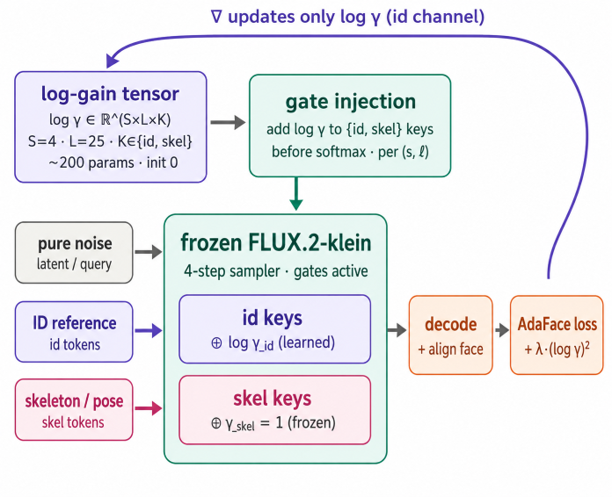
\includegraphics[width=\linewidth]{figures/rotate_id_gamma_gate.png}
\caption[Learned attention-budget allocator ($\gamma$-gate, Sec.~\ref{sec:learned})]{\textbf{Learned attention-budget allocator ($\gamma$-gate,
Sec.~\ref{sec:learned}).} A small \emph{log-gain tensor}
$\log\gamma\in\mathbb{R}^{S\times L\times K}$ ($S{=}4$ steps, $L{=}25$ layers,
$K{\in}\{\mathrm{id},\mathrm{skel}\}$; $\sim$200 params, initialized to $0$) is
injected into the frozen FLUX.2-klein sampler: at each step\,$s$ and layer\,$\ell$
it adds $\log\gamma_{s,\ell,k}$ to block $k$'s key columns \emph{before} softmax.
The identity-key gain is \emph{learned}; the skeleton-key gain is frozen at
$\gamma_{\mathrm{skel}}{=}1$, confining the change to identity. Trained
\emph{from pure noise} with the $4$-step sampler active, the decoded face is
detected, aligned, and scored by an AdaFace margin loss
$+\,\lambda\,\overline{(\log\gamma)^2}$; the gradient updates \emph{only}
$\log\gamma$ (the identity channel). The backbone is frozen throughout.}
\label{fig:allocator}
\end{figure}
